\documentclass[a4paper]{article}
\usepackage[czech]{babel}
\usepackage[utf8x]{inputenc}
\usepackage[T1]{fontenc}
\usepackage[plainpages=false,pdfpagelabels,unicode]{hyperref}
\usepackage{charter,graphicx}
\begin{document}
\title{Přehledová kapitola}
\maketitle
\section{Současný stav}

V současné době je vizualizace rozdělení disků při instalaci systému použita v minimu případů. Dále v kapitole rozeberu jednotlivé ukázky které jsem vybral, avšak souhrnně se dá říct, 
že instalátory se drží textového seznamu diskových oddílů uspořádaných do stromové struktury. Systémy jsem vybíral tak aby bylo možné porovnat alespoň nějakou vizuální stránku. Proto jsem vynechal
příklady typu Archlinux či Gentoo, které používají pouze instalaci z  příkazové řádky.  Dále pak uvedu pár příkladů vizualizace kterou používají nástroje na práci s disky jako je 
například program gparted.

\section{Příklady instalátorů - Linux}

\subsection{Debian}

Pro příklad jsem vybral 3 linuxové distribuce. Debian jakožto velmi konzervativní distribuci, udržující osvětčené postupy a programy, snažící se o maximální stabilitu i za cenu zastaralosti. 
Tato distribuce má grafický instalátor, spoléhá ovšem na zkušenosti a znalosti uživatele. K žádnému schematu se během instalace nedostaneme. Jak je vidět na obrázku č. 1, jediný způsob předání 
informace o plánovaném stavu disku je textový strom diskových oddílů obohacený o možnost výběru a ovládání myší.

\begin{figure}
\caption{Distribuce Debian}
\centering
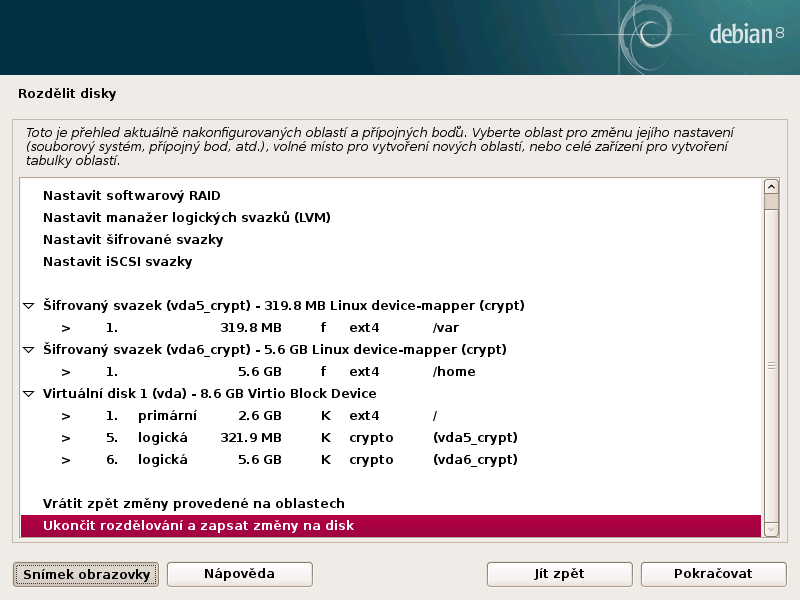
\includegraphics[width=.8\columnwidth]{pics/debian1.png}
\end{figure}

\subsection{Ubuntu}

Ubuntu linux je dalším příkladem, ač vychází z výše zmíněné distribuce Debian, instalátor používá svůj vlastní. Je také jediným zástupcem linuxové distribuce která využívá alespoň nějaké schéma 
pro znázornění stavu rozděleného disku. Dříve využívané schéma programu gparted bylo nahrazeno jednoduchou linkou v horní oblasti okna instalátoru. Na této lince jsou barevně znázorněny diskové 
oddíly vytvořené uživatelem. Stejné barvy jsou poté použity u každého ze záznamů v seznamu oddílů, jak je možné vidět na obrázku. Tento jednoduchý diagram umožňuje rychlý odhad poměrů různých 
částí které budou vytvořeny.

\begin{figure}
\label{fig:ubuntu}
\caption{Distribuce Ubuntu}
\centering
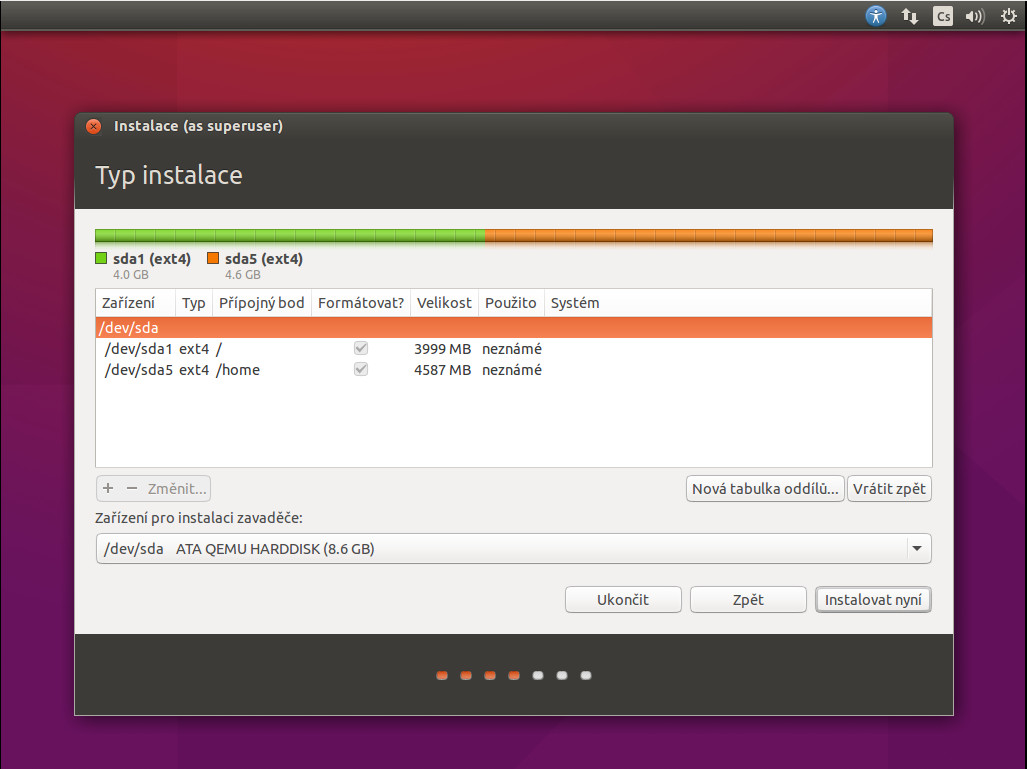
\includegraphics[width=.8\columnwidth]{pics/ubuntu1.jpg}
\end{figure}

\subsection{CentOS}

Jako příklad systémů které využívají instalátor Anaconda jsem vybral systém CentOS. Tato zkratka znamená Community ENterprise Operating System. Na svých stránkách uvádějí "The CentOS Linux
distribution is a stable, predictable, manageable and reproducible platform derived from the sources of Red Hat Enterprise Linux (RHEL)."[Citation needed] Jedná se v podstatě o systém Red Hat Enterprise 
Linux, ovšem bez podpory a opravných patchů od společnosti Red Hat. V současné době instalátor Anaconda používá též pouze textovou reprezentaci disku. Rozdíl oproti ostatním distribucím tvoří 
seznam změn který je zobrazen před finálním potvrzením a započetím formátování. Na obrázcích č. 3 a 4 můžeme vidět příklad tohoto seznamu. Situaci zpřehledňuje ale pouze pro malý počet změn. Seznam s 30 
záznamy o změnách je nepřehledný. Právě současný stav se snažím zlepšit v této práci.

\begin{figure}
\label{fig:centos1}
\caption{Distribuce CentOS}
\centering
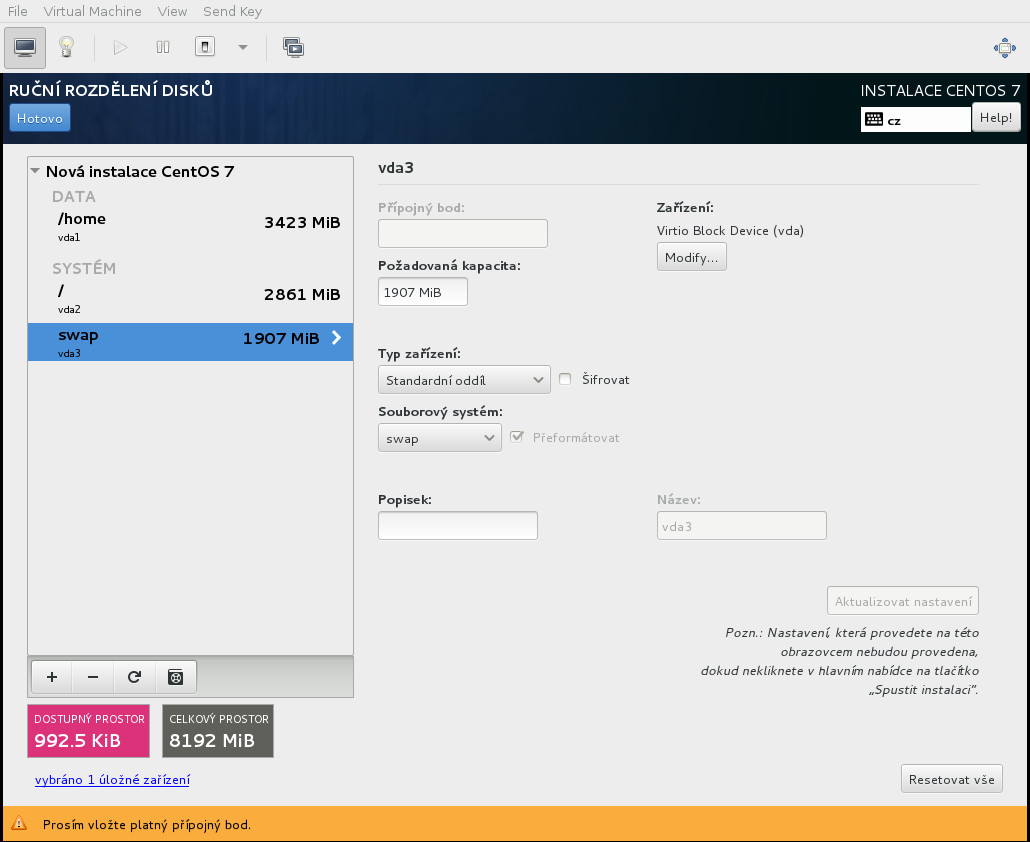
\includegraphics[width=.8\columnwidth]{pics/centos1.jpg}
\end{figure}

\begin{figure}
\label{fig:centos2}
\caption{Distribuce CentOS příklad souhrné tabulky}
\centering
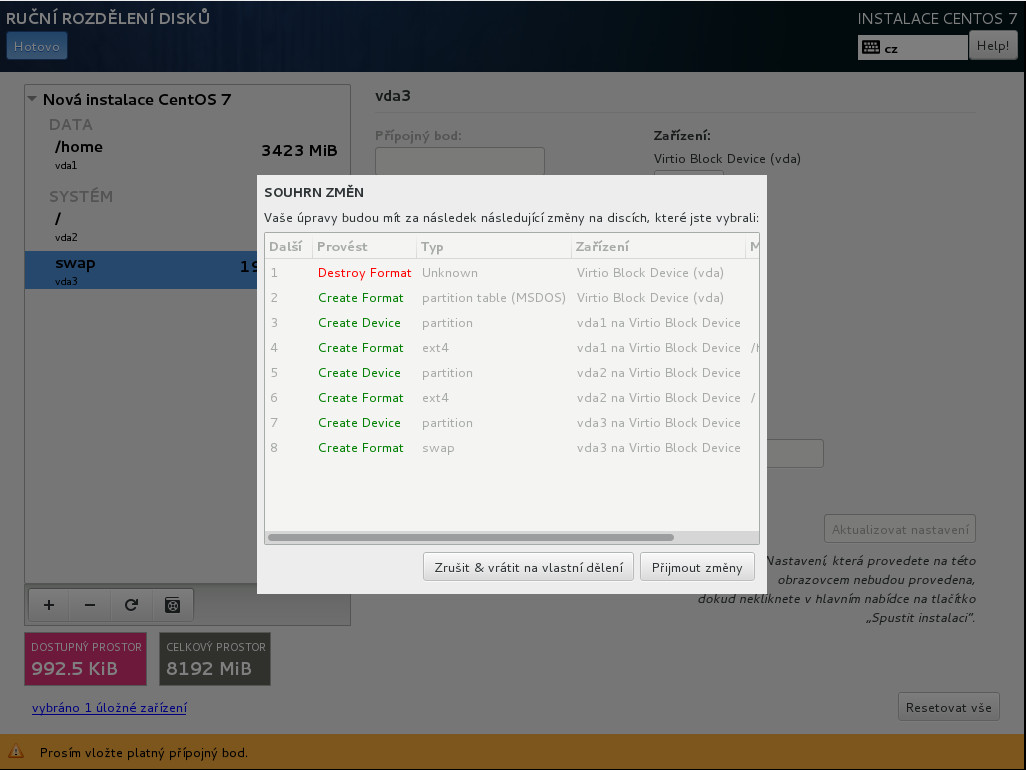
\includegraphics[width=.8\columnwidth]{pics/centos3.jpg}
\end{figure}

\subsection{Windows 10}

Pro srovnání uvádím i příklad nejrozšířenějšího systému, Windows. Vybral jsem, v současnosti nejrozšířenější verzi, Windows 10. Překvapivě se člověk ani zde nesetká s vizuálními pomůckami.
Tvůrci instalátoru spoléhají na automatickou instalaci a rozdělení disku s tím že pokročilou verzi s manuálním nastavováním zvolí uživatel který se vyzná i bez vodítek. V předchozích verzích
byl použit podobný přístup jako má instalátor distribuce Ubuntu, tj. obdélník znázorňující disk a barevné vyznačení oddílů.

\begin{figure}
\label{fig:win}
\caption{Systém Windows}
\centering
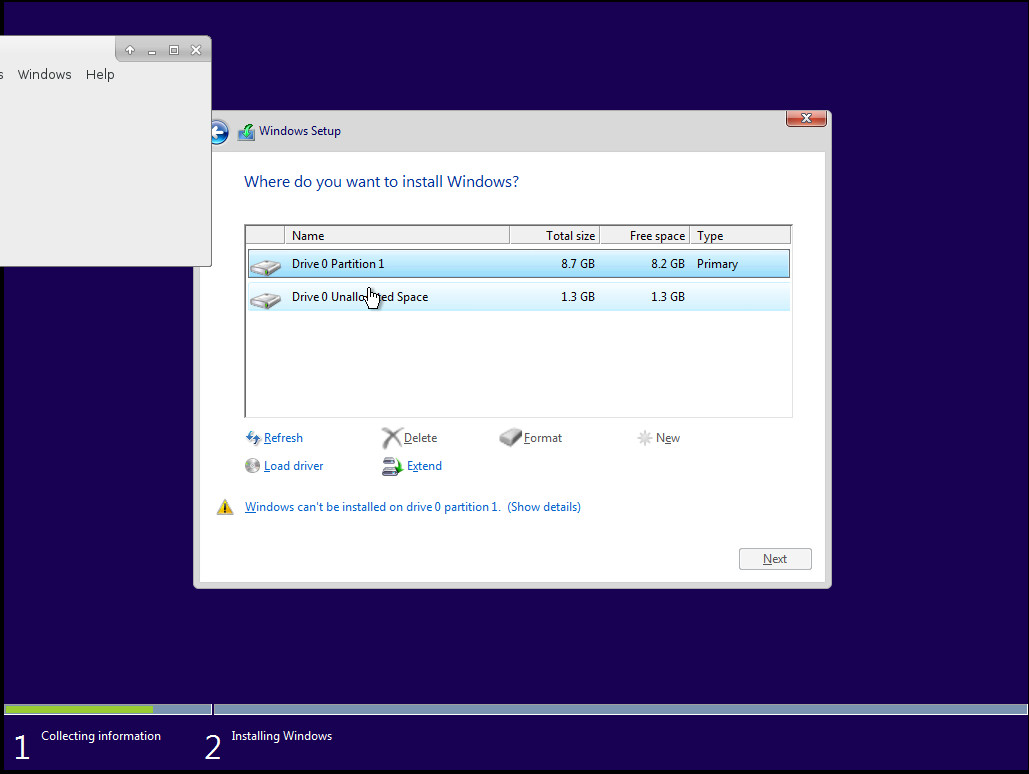
\includegraphics[width=.8\columnwidth]{pics/win1.jpg}
\end{figure}

\section{Programy sloužící pro manipulaci s disky}

\subsection{Gpatred}

Program Gparted je zástupcem programů které je možné spouštět i mimo fázi instalace systému. Dříve byl součástí instálátoru systému Ubuntu ale je možné jej spouštět i samostatně , například 
v případě potřeby zvětšovat úložné kapacitu virtuálních disků či disků jejichž souborový systém umožňuje pozdější modifikaci. Opět používá známé obdélníkové schéma. Každý disk je reprezentovaný 
obdélníkem a další informace jsou zobrazovány barevnými rámci uvnitř těchto obdélníků. Narozdíl od ostatních zmíněných programů obsahuje Gparted i grafické widgety pro manipulaci s disky 
a tím dosahuje efektu WYSIWYG editoru. Příkladem je widget pro zvětšení diskového oddílu který vidíme na obrázku číslo 6.

\begin{figure}
\label{fig:gparted}
\caption{Ukázka widgetu pro program Gparted}
\centering
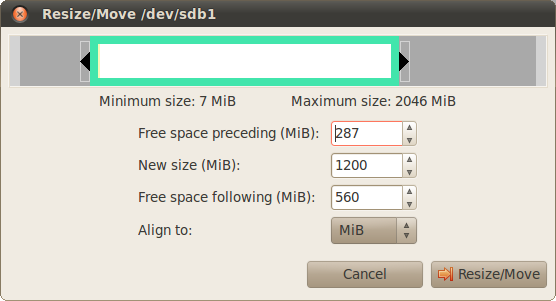
\includegraphics[width=.8\columnwidth]{pics/gparted-5-big.png}\\
\scriptsize Zdroj [Citation needed]
\end{figure}

\subsection{blivet-gui}

Posledním příkladem je program na manipulaci s disky který je součástí instalátoru Anaconda, využívá knihovnu nazvanou blivet stejně jako program kterým se zabývá tato práce. Autoři se zprvu 
rozhodli použít známé schéma avšak brzy narazili na problém s větším počtem disků a virtualizovanými disky. Na přiloženém obrázku vidíme že současné řešení je nedostatečné a použití grafu by
situaci zpřehlednilo. Jednotlivé úrovně barevných rámců budou znározněny samostatnými uzly grafu s hranami vyznačujícími vztahy mezi nimi. 

\begin{figure}
\label{fig:blivet}
\caption{Ukázka programu blivet-gui}
\centering
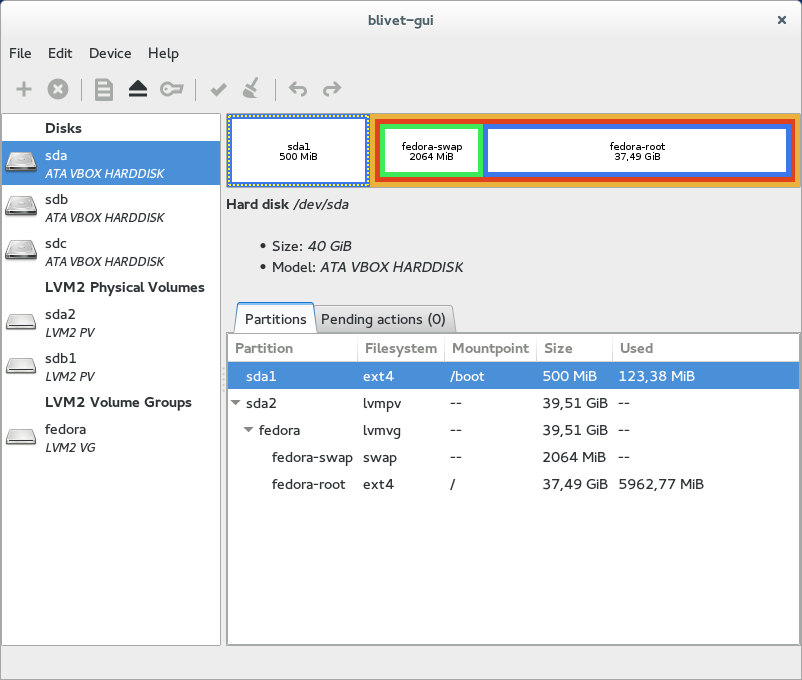
\includegraphics[width=.8\columnwidth]{pics/blivet-gui-1.png}\\
\scriptsize Zdroj [Citation needed]
\end{figure}
\end{document}
